%%%%%%%%%%%%%%%%%%%%%%%%%%%%%%%%%%%%%%%%%
% FRI Data Science_report LaTeX Template
% Version 1.0 (28/1/2020)
% 
% Jure Demšar (jure.demsar@fri.uni-lj.si)
%
% Based on MicromouseSymp article template by:
% Mathias Legrand (legrand.mathias@gmail.com) 
% With extensive modifications by:
% Antonio Valente (antonio.luis.valente@gmail.com)
%
% License:
% CC BY-NC-SA 3.0 (http://creativecommons.org/licenses/by-nc-sa/3.0/)
%
%%%%%%%%%%%%%%%%%%%%%%%%%%%%%%%%%%%%%%%%%


%----------------------------------------------------------------------------------------
%	PACKAGES AND OTHER DOCUMENT CONFIGURATIONS
%----------------------------------------------------------------------------------------
\documentclass[fleqn,moreauthors,10pt]{ds_report}
\usepackage[english]{babel}

\graphicspath{{fig/}}




%----------------------------------------------------------------------------------------
%	ARTICLE INFORMATION
%----------------------------------------------------------------------------------------

% Header
\JournalInfo{FRI Natural language processing course 2024}

% Interim or final report
\Archive{Project report} 
%\Archive{Final report} 

% Article title
\PaperTitle{Unsupervised Domain adaptation for Sentence Classification} 

% Authors (student competitors) and their info
\Authors{Veronika Matek, Karmen Frank and Luka Mihelič}

% Advisors
\affiliation{\textit{Advisors: Slavko Žitnik, Aleš Žagar, Boshko Koloski}}

% Keywords
\Keywords{Domain Adaptation, TSDAE, GPL, SBERT, Sentence Classification}
\newcommand{\keywordname}{Keywords}


%----------------------------------------------------------------------------------------
%	ABSTRACT
%----------------------------------------------------------------------------------------

\Abstract{
TO BE ADDED LATER IN PROCESS.
}

%----------------------------------------------------------------------------------------

\begin{document}

% Makes all text pages the same height
\flushbottom 

% Print the title and abstract box
\maketitle 

% Removes page numbering from the first page
\thispagestyle{empty} 

%----------------------------------------------------------------------------------------
%	ARTICLE CONTENTS
%----------------------------------------------------------------------------------------

\section*{Introduction}

\iffalse	
	Uvodni zapis - slabosti SBERT-a in podobnih metod, zakaj se uporablja TSDAE in GPL (v povezavi s prilagoditvijo domene). Osredotočili se bomo na "domain adaptation" za slovenski jezik, pri čemer bomo metode testirali nad problemom "sentimental analysis" (nekako povežemo besedilo na problem klasifikacija pri čustvih). Cilj projekta je bila implementacija metod TSDAE, GPL, s katerimi finetunamo SBERT (BERT+pooling), in testiranje metod ter primerjava rezultatov nad problemom klasifikacije stavkov v eno izmed "pos", "neg", "neutral". Opazovali smo tudi izbrane parametre tekom učenja posameznega pristopa.

	In the Introduction section you should write about the
	relevance of your work (what is the purpose of the project,
	what will we solve) and about related work (what solutions
	for the problem already exist). Where appropriate, reference
	scientific work conducted by other researchers.
\fi

Previous state-of-the-art methods, like SBERT, for deriving sentence embeddings have a key problem of not working for specific topics and domains. We bypass this problem by additionally fine-tuning our non-domain-specific base model using methods like TSDAE and GPL. Both of the methods have been proven to significantly outperform previous state-of-the-art models, like Masked Language Model, on domain specific training data, working even better if combined together~\cite{wang-etal-2021-tsdae-using, GPL}. 

Most of these previous successful methods were trained on Semantic Textual Similarity, which does not take into account any domain knowledge. Some examples of these approaches are SBERT and Infersent. One such reason for the lack of domain knowledge is that training a model might require a lot of labeled data, which can be expensive and hard to get. This holds true especially for specific topics. One way of solving this is training the model on the general corpus before fine-tuning it to the required domain~\cite{wang-etal-2021-tsdae-using, GPL}.

In this report we aim to fine-tune an unsupervised multilingual base model SBERT with two of the mentioned domain adaptation techniques, namely Transformer-based Sequential Denoising Auto-Encoder (TSDAE) and Generative Pseudo Labeling (GPL) on the SentiNews classification dataset. We classify Slovenian sentences based on their sentiment, which can be positive, neutral or negative. We compare the results given by the pretrained base model and by the base model fine-tuned with both mentioned methods as well as a combination of them. 

We observe any improvement when faced with domain specific data compared to SBERT, trained on the exact same input sentences. We also distinguish the impact of different parameters during the learning of each approach and try to find the optimums.



%------------------------------------------------



\section*{Methods}

\iffalse	
Use the Methods section to describe what you did an how you did it -- in what way did you prepare the data, what algorithms did you use, how did you test various solutions ... Provide all the required details for a reproduction of your work.

Tu nekoliko opišemo SBERT - predvsem glede sentence embeddingov, ki jih potrebujemo za naprej.
\fi

\subsection*{SBERT}
SBERT (Sentence Bidirectional Encoder Representations from Transformers) adds siamese and triplet structure networks to the pre-trained transformer network BERT, which produces state-of-the-art results for natural language processing tasks such as question answering, sentence classification and sentence-pair regression. SBERT applies a pooling layer to the output of a BERT/RoBERTa model, deriving fixed sized sentence embeddings. With the added network structures we can fine-tune the model and update weights so the to output results are sentence embeddings that are semantically meaningful \cite{SBERT}. Semantic aspects embedded in the continuous vector space can be measured with the cosine metric similarity, where similar semantic representations in a high-dimensional vector space are closer to each other. The available training data for a given knowledge domain also defines the SBERT network structure. Therefore we may use the classification, regression or the triplet objective function for different kind of tasks.

The classification objective function concatenates sentence embeddings \(u\) and \(v\) with the element-wise difference \(|u - v|\) and multiplies it with the trainable weight \( W_t \in \mathbb{R}^{3n \times k} \) \cite{SBERT}:

\begin{equation}
o = \text{softmax}(W_t(u, v, |u - v|)) \text{,}
\label{eq:softmax}
\end{equation}

where $n$ is the sentence embeddings' dimension and $k$ number of labels.


\subsection*{TSDAE}

Transformer-based Sequential Denoising Auto-Encoder (TSDAE) is a state-of-the-art unsupervised method used for domain adaptation with an encoder-decoder architecture. A shortcoming of previous sentence embedding techniques like SBERT is the lack of domain knowledge. Fine-tuning a model like this with TSDAE can adapt our model to a specific domain without any labeled data, as this is hard and expensive to acquire~\cite{wang-etal-2021-tsdae-using}. 

Before training the model, TSDAE corrupts the input sentences, for example by deleting or swapping words, and encodes them to a fixed size vector. The goal of the decoder is to reconstruct the vectors of the original input by prediciting what was changed. It is important to note that the decoder has no context as it doesn't have access to other sentence embeddings and thus creates a bottleneck~\cite{wang-etal-2021-tsdae-using}. This architecture can be seen in Figure~\ref{fig:tsdae}.

\begin{figure}[ht]\centering
	\vspace{12 pt}
	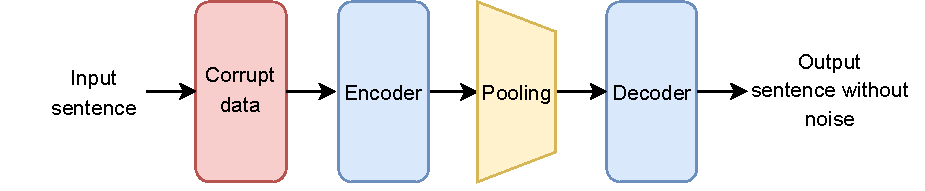
\includegraphics[width=\linewidth]{TSDAE_scheme.pdf}
	\vspace{5 pt}
	\caption{Workflow of TSDAE. The input sentences are first corrupted and then encoded into fixed size vectors. The vectors are pooled and then attempted to be reconstructed with the decoder.}
	\label{fig:tsdae}
\end{figure}

For the purpose of classifying Slovenian sentences based on their sentiment we fine-tune the SBERT model with TSDAE. We choose bert-base-uncased (TODO: change base model accordingly) for our base model. During training we use the DenoisingAutoEncoderLoss as our loss function, which expects pairs of original and corrupted sentences as the input. We train the model where the decoder attempts the reconstruction of the corrupted sentences and compare our results with the corpus~\cite{SentenceTransformers}.

% TSDAE has been shown by Wang, Reimers and Gurevych \cite{wang-etal-2021-tsdae-using} to outperform other unsupervised approaches and other supervised models, trained with a lot of labeled data. Many previous works were evaluated on Semantic Textual Similarity (STS) which might return good performance but it is unclear how it performs on specific domains \cite{wang-etal-2021-tsdae-using}.


\subsection*{GPL}

The Generative Pseudo Labeling (GPL) is a domain adaptation technique that utilizes unsupervised learning. It allows us to fine-tune a dense retrieval model (for example SBERT \cite{SBERT}) on a desired domain. First step of GPL is preparing (query, sentence)-pairs. This takes three phases: generating suitable queries, negative mining and using cross-encoder to assign a score to each pair \cite{GPL}. This process is visualised in Figure~\ref{fig:GPL}.

\begin{figure}[ht]\centering
	\vspace{12 pt}
	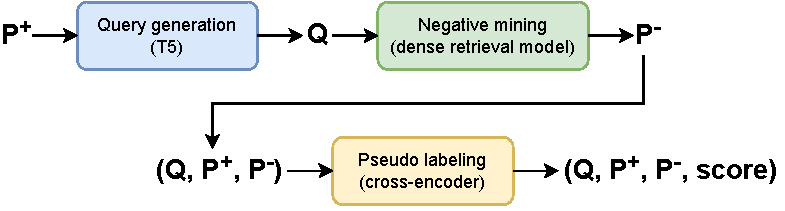
\includegraphics[width=\linewidth]{GPL_data_preprocessing.pdf}
	\vspace{5 pt}
	\caption{The workflow of GPL's sentence preparation step. Queries $Q$ are generated for each input sentence $P^{+}$. The generated queries are then used for negative mining or finding similar sentences $P^{-}$. Pseudo labeling step involves a cross-encoder that assigns a score to each (query, sentence)-pair.}
	\label{fig:GPL}
\end{figure}

Queries are generated using a pretrained T5 encoder-decoder model \cite{T5}. Three queries are generated for each input sentence. The next step is negative mining, where 50 of the most similar sentences are retrieved for each of the generated queries, using an existing dense retrieval model. The (query, input sentence)-pairs are denoted as $(Q, P^{+})$ and the negative sentence as $P^{-}$.

The last step of data preparation involves a cross-encoder that assigns a score to each (query, sentence)-pair. For each $(Q, P^{+}, P^{-})$-tuple a margin $\delta$ is calculated using the next equation:
\begin{equation}
	\delta = \text{CE}(Q, P^{+}) - \text{CE}(Q, P^{-})\text{,}
\label{eq:delta}
\end{equation}
where $CE$ is the score predicted by the cross-encoder. This gives us a dataset $D_{GPL} = {\{ ( Q_i, P_i, P_i^{-}, \delta_i ) \}}_i$, which is used for training a dense retrieval model with the MarginMSE loss function. This model thus learns to map queries and sentences into a vector space and is fine-tuned to a given domain.

The MarginMSE loss \cite{marginMSE} relies on the scores, or pseudo labels, provided by the cross-encoder. It teaches the dense retrieval model to predict the margin between the score of $(Q, P^{+})$-pair and score of $(Q, P^{-})$-pair. It follows the next equation:
\begin{equation}
	\text{MarginMSE} = \frac{1}{N} \sum_{i=0}^{N-1} |\hat{\delta_i} - \delta_i|^{2} \text{,}
\label{eq:delta}
\end{equation}
where $N$ is the batch size, $\delta_i$ is defined in equation~\ref{eq:delta}, provided by the cross-encoder, and $\hat{\delta_i}$ is derived by the (student) dense retrieval model, which we are fine-tuning.


\subsection*{Data}
We used the SentiNews dataset \cite{sentiNews}, which contains 169k sentences from 10.4k documents, equiped with sentiment labels, in the Slovenian language. A few examples of dataset's elements are shown in Table~\ref{tab1}.

\begin{table}[!h]
	\footnotesize
	\begin{center}
		\begin{tabular}{ |c|c| } 
		\hline
		Sentence & Sentiment \\
		\hline
		
		Kaže, da se blejskim vilam vendarle obeta lepša prihodnost. & positive \\
		O tem bo Evropska komisija odločala septembra. &neutral\\
		V Sloveniji je ta rast znašala sedem odstotkov. &negative\\
		
		\hline
		\end{tabular}
	\end{center}
\caption{Examples from the SentiNews \cite{sentiNews} dataset.}
\label{tab1}
\end{table}

The dataset was split into train, validation and test set (TO DO). For each method we use to fine-tune the base model, the exact same datasets are used.
Kakšne podatke uporabljamo, kako izgledajo, in what way did you prepare the data, delitev na množice (poudarimo, da se vse metode treniranjo z enako učno množico).
Pokažemo morda par primerov povedi v tabeli.


\subsection*{Testing approach}
Naslov morda še ni ustrezen in se bo prilagodil.
Katero metriko uporabimo za primerjavo rezultatov, kako iz sentence embedding pridemo do klasifikacije povedi.



%------------------------------------------------



\section*{Results}

TO DO:
Use the results section to present the final results of your work. Present the results in a objective and scientific fashion. Use visualisations to convey your results in a clear and efficient manner. When comparing results between various techniques use appropriate statistical methodology.



%------------------------------------------------



\section*{Discussion}

TO DO:
Use the Discussion section to objectively evaluate your work, do not just put praise on everything you did, be critical and exposes flaws and weaknesses of your solution. You can also explain what you would do differently if you would be able to start again and what upgrades could be done on the project in the future.



%------------------------------------------------



\section*{Acknowledgments}

Here you can thank other persons (advisors, colleagues ...) that contributed to the successful completion of your project.


%----------------------------------------------------------------------------------------
%	REFERENCE LIST
%----------------------------------------------------------------------------------------
\bibliographystyle{unsrt}
\bibliography{report}


\end{document}
